\documentclass[a4paper,10pt]{report}
\usepackage[utf8x]{inputenc}
\usepackage{url}

\usepackage{titling}
\usepackage{amsmath}
\usepackage{amssymb}
\usepackage{graphicx}
\usepackage{listings}
\usepackage{caption}
\usepackage{subcaption}
\usepackage{textcomp}

\usepackage{algpseudocode}
\usepackage{algorithm}

%use either 3 or 4 (or 5 if needed)
\setcounter{secnumdepth}{3}
\setcounter{tocdepth}{3}

\bibliographystyle{vancouver.bst}

% Title Page
\pretitle{\begin{center}\Huge CS344 - Final Report \end{center}\begin{center}}
\title{\Huge Smart Phone Cryptography}
\posttitle{\end{center}\begin{center}\LARGE A comparison of techniques for encrypted data communication \end{center}}


\preauthor{\begin{center}\LARGE Tom Nicholls - 1006007\end{center}\begin{center}}
\author{Discrete Mathematics - Year 3}
\postauthor{\end{center}\begin{center}\large Marcin Jurdzinski\end{center}}

\begin{document}
\maketitle

\begin{abstract}
%Should be 200 words - check before final proof read

Protecting sensitive or secret information has always been an important issue. With the increased popularity and usability of smartphones, tasks from accessing confidential work files or personal bank accounts to communicating with clients and friends, are being completed through applications over mobile or wireless internet connections. In this project the various cryptographic schemes used by popular applications available to Android based smartphones for secure data communication will be researched. Accompanying this will be a study of other cryptographic schemes. These techniques will be implemented through a data transmission application. Tests will be carried out to analyse various important factors that need to be considered for a successful encrypted data transmission application. An original conclusion will then be drawn as to whether the current techniques of cryptography available are appropriate or if a new scheme should be encouraged. The results of the described implementation and analysis were that the currently used cryptographic techniques are appropriate for the current state of smartphone usage and capabilities. These techniques, however, should be combined to create a new application. A different technique, which has increased security for a smaller resource cost, exists that can easily be used in the event that the requirements of the current cryptographic schemes surpass the available resources of current smartphones. 

{\bf Keywords:} Cryptography, Encryption, Decryption, Smartphone, Android, AES, RSA, ECC
\end{abstract}

\tableofcontents


\chapter{Introduction}


\section{Background}

To start this project report, all relevant background information will be presented allowing the reader to fully understand all aspects of the project. An overview of basic techniques and topics will be given, with a greater explanation for more specialised areas. 

\subsection{Smartphones}

In this section, the basics of the smartphone will be introduced and described. As smartphones are a prominent part of modern culture, and therefore known in some degree to everybody, only an overview will be given. The book by Sarah Allen et al. \cite{whatisasmartphone} was used as reference material.

'Mobile' or 'Cell' phones have been available for commercial use since the beginning of the 1980s. The most popular functions of these phones are for telephone calls, text or multi-media message sending or even basic internet access and games. With the development of the smartphone these older devices are considered low-end phones. Higher-end phones, universally named the 'smartphone' provide the same basic features (telephone calls, messaging etc) but with a plethora of added functions such as full internet access, as well as increased computing capabilities through more powerful processors and other hardware. Smartphones also utilise the QWERTY keyboard and a larger, higher-resolution, screen. 

Compared to desktop computers, smartphones have a diverse set of operating systems, determined by the manufacturer of the smartphone. Smartphone operating systems include; Apple iPhone iOS \cite{appleios}, Windows Phone \cite{windowsphone} and Google Android \cite{googleandroid}. Each operating system, unlike that of a desktop, determines which programming language a developer must use if they are to develop an app for a particular smartphone. This leads to a separate application marketplace, a database where users can download and install new applications, for each smartphone operating system. Whilst applications can be developed in a cross-platform manner, through the use of HTML and CSS, this is not yet standard, so the various marketplaces are individual in the applications that are on offer. The Android operating system, developed by Google and mostly found on devices by Samsung, HTC or Google themselves, use the Google Play marketplace \cite{googleplay} for application distribution with applications being developed using the Java programming language.

The message sending capabilities of smartphones is the feature that is most important for this project, whether it be using the in-built short messaging service (SMS) or through the use of an installed application. Message sending allows the specification of a recipient and a user entered message for that recipient, with a near instant sending and receiving of that message. On average, the message is of a short length and can be described as an easier, more lightweight form of simple email exchange. 

\subsection{Cryptography}

Taken from the book by Richard A. Mollin \cite{richardmollin}, the meaning of cryptography is 'the study of methods for sending messages in secret (namely, in enciphered or disguised form) so that only the intended recipient can remove the disguise and read the message (or decipher it).' Many keywords are used in the study of cryptography and help to give an introduction to the field; 

\begin{itemize}
 \item Plaintext - The original message, input by the initiating user.
 \item Ciphertext - The disguised message, created using the plaintext.
 \item Encryption - The process of transforming the plaintext into the ciphertext.
 \item Decryption - The process of turning the ciphertext into the original plaintext. Accomplished by the recipient, who has the knowledge to remove the disguise.
 \item Cipher - The Method for enciphering and deciphering.
 \item Cryptanalysis - The study of mathematical techniques for attempting to break the cryptographic methods.
 \item Cryptographic Key - A tool for encryption or decryption
\end{itemize}

\noindent
This shows that basic cryptography has the following form:

\begin{center}

  \textbf{Plaintext} $\rightarrow$ \emph{Encryption} $\rightsquigarrow$ \textbf{Ciphertext} $\rightsquigarrow$ \emph{Decryption} $\rightarrow$ \textbf{Plaintext}

\end{center}

\noindent
Two very basic examples of cryptography, which can and have been expanded into many different, more elaborate, techniques, are the substitution and transposition ciphers. Substitution ciphers replace symbols in the plaintext with other symbols, using a given rule (the key), to produce the ciphertext. For example, the key may be; a $\rightarrow$ q, b $\rightarrow$  f, c $\rightarrow$  m, and so on. A transposition cipher, on the other hand, transposes the places in which the plaintext letters are situated. This means that no new letters are introduced. The key for this cipher is a permutation that describes how the letters should be transposed. For a plaintext that consists of 10 letters, the key could be:

\begin{center}
$
\begin{pmatrix}
  1 & 2 & 3 & 4 & 5 & 6 & 7 & 8 & 9 & 10 \\
  1 & 2 & 5 & 7 & 6 & 4 & 9 & 10 & 3 & 8
 \end{pmatrix}
$
\end{center}

where the symbol in the position number in the top row, is replaced by the symbol in the position number below it (in the second row). Using these techniques as a basis, other more advanced cryptographic schemes can be created and are defined by the cipher (and key) that is used for the particular method.

Cryptography has been used in some form or another to exchange secret message throughout history. For example, the first use of of cryptography in a military setting was by the Spartans in 475 B.C. In the modern age, cryptography is most commonly used when sending or storing data using a computer system, such as sending an email across a network, or saving a file on a company server. 

\section{Motivation}

Protecting important and secret information is big issue, particularly when data such as bank accounts details or private work related conversations are taking place or being exchanged. When new devices or computer systems are developed and deployed, the security of that system is always considered and studied. Smartphones, on the other hand, have a substantial amount of user-input in the form of publicly developed applications. With smartphones becoming the most popular tool for communicating and completing other tasks with the transfer of sensitive information combined with the fact that there are a vast number of tools for completing such tasks, the study of the strength and current state of security of smartphones is an ever evolving field. This creates a number of questions, the answers to which form the basis of this project:

\begin{itemize}
 \item Do applications that facilitate the secure transfer of messages exist?
 \item What are the cryptographic techniques behind these applications?
 \item Are there other techniques which could also be used for this purpose?
 \item What is the performance of these styles applications?
 \item Can these applications or methods be improved upon?
 \item Can a conclusion be made about the current state of secure message communication and its future? 
\end{itemize}

The results of this project will contribute an original conclusion to the field of cryptography within smartphones. Preliminary research showed that the questions set out to be answered in this project have not been answered before for the current, present-day state of smartphones. This is important because even in the last few years significant improvements and developments have been made concerning the design and processing power of smartphones which has had a tremendous affect on smartphone usability, for example the more advanced and widely available use of GPS in direction planning. 

\section{Scope and Limitations}

It is important to set out in the introduction to this project report what the scope of the project is and to describe any limitations that have been placed on the project.

Firstly, as will be detailed later in this report, the choice was made that any developed software will be in the Java programming language and that the Android operating system will be the focus of study and application development. This is so that the project can be accomplished within the given time frame, to the standard required and with the hardware that is more easily available. It also ensures that the project does to try to encompass an area that is so huge that any conclusion loses focus and therefore its value.

This project also focuses on the use of cryptography in sending secure messages between users as opposed to other issues regarding smartphone security. A few examples of other forms of security related to smartphones could be a study of stored data protection, techniques to retrieve data from a smartphone wirelessly and protecting a smartphone from attacks or viruses. The reasons that this project is focused on one particular aspect of security with smartphones is much that same as the reasons given for the previous point. Furthermore, narrowing the scope of the project in this way means that a full solution and conclusion can be found for this particular aspect, as opposed to giving brief or vague conclusions for a number of aspects. Cryptography, particularly in this setting, also allows for a project that encompasses both computer science and mathematics and therefore is appropriate for a Discrete Mathematics student. 

Lastly, this goal of this project is not to design and develop a product (application) that meets industry and user requires and can be sold or released to the general public. A project of that type would focus more on human-computer interactions, product design and marketing, as opposed to focusing on the mathematically based computer science areas of smartphones and cryptography. Therefore, the project can be categorised as a combination of both a research based and software development based project, each emphasising and reinforcing the other. 

\section{Issues}

Every project is faced with issues regarding the projects final goals and outcomes, or the techniques or methods used to reach these outcomes. This section will discuss the issues faced or considered with this project. 

\subsection{Legal}

Legal issues are the main issues that need to be considered with this project. As a large section of this project is research based, it needs to be ensured that all materials used are correctly and appropriately referenced. Furthermore, as this project is centred on the issues of computer security, in the form of cryptography, legal issues need to be discussed \cite{dataprotect} \cite{internetlaw}. As long as any material that is encrypted is legal in its own rights and that only data that is solely owned by myself is used in the cryptographic processes, then any legal issues will be avoided in this case. Also, the resulting product facilitates the secure communication of messages which, in the wrong hands, could be used to aid a number of illegal operations. To avoid the direct use of the final application for illegal purposes, it will not be published to the Google Play application marketplace and will therefore not be available to the public. This also means that a disclaimer or end-user license agreement (EULA) will not be required, which would included the consultation of a professional lawyer. If the software created in this project was obtained by a malicious user, then any data required by the police could and would be given to break the illegal encryption by the author \cite{pcworldart}.

\subsection{Ethical}

In almost all modern technical advances, ethical issues can be found, posing unique problems depending on the perception or views of the topic by various groups or persons. For this topic, the legal issues presented above can also be viewed as ethical issues. Should an application be developed, or a field be advanced, that could be used to facilitate illegal operations? This question, and many like it, could and are constantly discussed and argued by professionals and amateurs alike, from almost all academic backgrounds. Because of this, a universally agreed upon set of ethics will never be concretely reached. However, through the actions taken to escape any legal issues, the avoidance of any major ethical issues are avoided. 

As no interviews, questionnaires or experiments will be taken place in this project, other ethical issues regarding this do not need to be considered. 

\subsection{Social and Professional}

With smartphones and text messaging services already being a central part of society, this project does not face any social issues. %not really sure where to go from here or what to talk about for professional issues

\section{Report Structure}

The structure of the report from this point onwards will be as follows:

\begin{description}
  \item[Objectives] A discussion of the objectives and goals of the project.
  \item[Research] Presentation and thorough explanation of all research completed.
  \item[Design] Full system design, outlining and explaining choices made and tools used. 
  \item[Development] Implementation and software development aspect of the project presented, including the testing phase.
  \item[Results] Analysis of the developed system accompanied with all conclusions and results found. 
  \item[Further Work] All further work completed for this project and a suggestion and discussion of any improvements that could be made.
  \item[Project Conclusion] A conclusion of the project as a whole, including self-assessment.
  \item[Acknowledgements] A list of acknowledgements relating to this project.
  \item[References] All reference material used through the project.
\end{description}

Theorems, proofs, code snippets, diagrams and screen shots will be used throughout, as required, to improve understanding and to help explain various sections of this report. 


\chapter{Objectives} %Could be expanded upon???

In order to answer the questions described previously, certain goals and objectives must be met. The main objectives of this project where: 

\begin{enumerate}
  \item Research
  \begin{itemize}
    \item Framework design
    \item Currently Available Applications
    \item Cryptographic Techniques
    \item Relevant factors that can be used to compare schemes implemented on a mobile device
  \end{itemize}
  \item Development
  \begin{itemize}
    \item Framework
    \begin{itemize} 
      \item Design Data Communication framework
      \begin{itemize}
        \item Server
        \item Mobile Application
        \item P.C Client
      \end{itemize}
    \end{itemize}
  \item Encrypted Data Communication
  \begin{itemize}
    \item Design and implement cryptographic techniques
  \end{itemize}
  \end{itemize}
  \item Analysis
  \begin{itemize}
    \item Perform tests from research
    \item Collect and present results
  \end{itemize}
  \item Conclusion
  \begin{itemize}
    \item Present and justify the findings and conclusions that can be made form the completed tests
    \item Show possible adjustments to the implemented schemes which would increase their usability
  \end{itemize}
  \item Further Work
  \begin{itemize}
    \item Detail possible extensions that can be made to the systems to include other possible functions
  \end{itemize}
\end{enumerate}

All aspects of software development are accompanied by thorough testing and are completed using a test driven development technique in a plan-driven setting, as described by Ian Sommerville \cite{iansommerville}. A further breakdown of the objectives, together with a thorough project task timetable, can be found in the form of a Gantt chart in Appendix \ref{A}.

\chapter{Research}

All completed research will now be presented, corresponding with the goals included in the Objectives section of this report. 

\section{Framework}

The system framework refers to the developed software that will facilitate the communication of data messages between any two users of the system, whilst not including any form of encryption or decryption. The research required to design a system framework was fairly minimal as most aspects of the software development for this project has already been covered, however how a full system should be set up had not. As the Java programming language had already been determined as the language that would be used in this project, the finer points of data communication required research. Android application development in this setting, along with how user data should be stored, also required some research. 

\subsection{System setup}

%big java book - multi client server
%possibly add to this when back at uni
%add in multi-threading etc

The backbone of the developed system was the sending and receiving of data messages between two clients. An initial approach could be that a client, be it a P.C or Android application based client, would send the user input message directly to the recipient. This, however, would required a constant link between all clients of the system, which is not practical due to users having different access habits or varied availability. It also requires a lot more computational power and resources, as each client has to track and directly communicate with each other client, which also is very fragile and prone to errors. Another approach, the approach used in this project, was found whilst researching using the book by Daniel Liang \cite{ydanielliang}. The method revolves around the development or a central server, which can be connected to by clients of the system, also known as a multi-client server. Data messages can then be sent to the server by each client, accompanied by the user ID of the intended recipient of the message. This message is then saved and can be sent to the intended user the next time the user logs on to the system or, if the user is already logged on to the system, the next time they 'refresh', asking the server to send any new messages. This is a slight adaptation to the method described by the reference material, which describes each communication link be created as a separate 'session' but, as with the initial approach, requires both users to be logged on to the system at the same time and simulates a more 'instant' messaging service. The adaptation to the researched method allows users to send and retrieve messages independently and is a more practical approach. This is particularly more practical for smartphone users where connection to the internet or a server can be indeterminate. Consideration was made as to how more than two users of the system could simultaneously communicate, but it was decided that as this is a feature not present in standard, unencrypted message communication for smartphones, it would not be required for this developed system. Utilising a central server creates a much more robust system, as the server will not be prone to failure (due to the nature of a server) and has the resources to handle almost all of the data management and tasks required for the system to function, as opposed to forcing the clients to complete this computation. It also acts as the central point of the system, allowing for development and updates to be made without a complete overhaul of the system. 

%add diagram from book

\subsection{Data Communication}

%networking book - sockets - have a look through for ideas
The book 'An Introduction to Network Programming with Java' \cite{javanetworking} was used as reference material for this section of research. 

The two main entities used in network communications are ports and sockets. A port is a dedicated logical connection to a particular server or service across a network. This, however, has no relation to the number of physical connections to the specified computer, which is normally only one. Ports in the range 1-1023 are normally reserved for specified standard services. For example, port 80 is normally used by Web servers. Ports 1024-65535 are not reserved or for non-standard services so can therefore be used for network application programming. When a connection to a particular server program is attempted by a user, the host machine address and server port number is provided. The transmission is then passed to the appropriate service that is waiting for requests. For the majority of applications, multiple users are likely to request communication access at the same time. To keep the communication dialogues separate, sockets are used. As with ports, sockets are an abstract concept and not a physical piece of hardware. Sockets are used to indicate each end-point of a communication link between two processes. Once a communication request has been established for the particular port, the server and client will each create their socket, dedicated for the communication of data for that purpose. The sockets used are described as TCP/IP sockets as they follow the Transmission Control Protocol, a higher level protocol placed over the Internet Protocol. This link is therefore connection-orientated which, although slower, is more reliable than the connectionless User Datagram Protocol (UDP) based sockets. Data, in the form of characters or files, can be transmitted across this link using data streams, which 'feed' the data through the sockets to the recipient, be it the client or the server. Acknowledgement files will be implemented to check that the correct data has been sent and received.

\subsection{Android Application}

%android developers and android book

With the availability of various resources \cite{androiddevelopers} \cite{markogargenta}, the research into android application development for this project could be completed efficiently. Although various methods for data communication with android applications existed, it was found that socket-based network programming could be used in the same was as for P.C clients (as described above). Other methods involved using HTTP Get and Post commands, a completely different technique to that used for the P.C based clients. Using the same technique for both clients was the logical choice for the development of the framework for this project.

Data compatibility between the clients will be ensured through the use of the Extensible Markup Language (XML) file structure. This file structure can be received and parsed by software developed for both platforms. 'A typical xml document contains sequences of nested tags describing and evaluating a multitude of objects and structures without any constraints, apart from those imposed by basic xml grammar' \cite{xmlbook}. The hierarchy of the information contained in an XML document can be accurately and correctly shown through the creation of a conceptual data tree. This allows the XML document to be precisely and efficiently parsed.

\begin{figure}[htb]
\centering
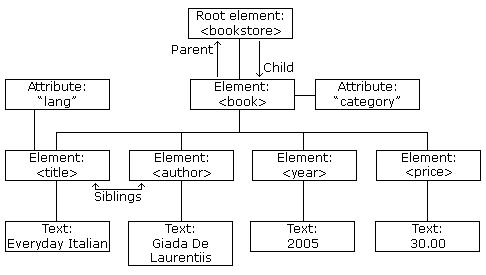
\includegraphics[scale=0.4]{images/nodetree.jpg}
\vspace{-10pt}
\caption{Tree structure representing an XML file for a bookstore.}
\vspace{-10pt}
\label{fig:exampleimg1}
\end{figure}

\begin{figure}[htb]
\centering
\lstinputlisting[basicstyle=\ttfamily\scriptsize]{documents/xmlexample.xml}
\vspace{-10pt}
\caption{The corresponding XML file for a bookstore.}
\label{fig:xml}
\end{figure}

An example, taken from w3schools.com \cite{w3schoolsxmlexample}, of a basic XML document more clearly shows the structure and formatting used. Figure \ref{fig:exampleimg1} and Figure \ref{fig:xml} show that $<$bookstore$>$ is the root element of the document, and that all $<$book$>$ elements are contained within $<$bookstore$>$. The book element has 4 'children': $<$title$>$, $<$author$>$, $<$year$>$ and $<$price$>$. These children as used to describe and give properties to the associated book. Within this project, the XML files will be set out quite similar, with the full document set up displayed in the design section of this report. 

\subsection{Data Storage}

%mysql - website and book - look for ideas
In order to store and manage the data for each user (I.D, encryption information, messages), MySQL \cite{mysql} will be used. MySQL is the most popular and highly used open source relational database management system (RDBMS). It provides user access to a server which hosts a number of databases. This server can be set up locally on through an external provider. In order to connect, access and edit the database through the developed system, JDBC will be used. 'JDBC is a set of programming APIs that allows easy connection to a wide range of databases (especially relational databases) through Java programs' \cite{jdbcmysql}. JDBC programming involves creating and executing SQL queries or 'statements' and processing the returned ResultSet objects. Statements contain the commands to select or edit particular entries in the database. A full description of the design of the database system in this project will be included in the following chapter. 

\section{Available Applications}

The research completed into the applications for encrypted message transfer that are currently available will now be presented. The two 'non-standard' applications were the only applications that could be found on the google play marketplace \cite{googleplay} through the use of various related search keywords. Most applications that where returned focused on encrypting stored data on the smarphone, as opposed to encrypting messages for sending or receiving, showing that there is a requirement in the market for more secure message communication applications. A full explanation and study of the relevant encryption methods will be displayed in the next section.

\subsection{Short Messaging Service}

The short messaging service is a text messaging service featured on all makes and models of mobile and smart phone. The user enters the recipients mobile telephone number and can send a short message (of only text) to the recipient. These messages are encrypted between the phone and base station however, it is required by law that government enforcement agencies can and should be able to conduct lawful surveillance of SMS messages when required \cite{aresmssafe}. Because of this, unlawful access to SMS messages is possible, by means other than actually breaking the encryption on the messages.

\subsection{Cloak SMS}

Cloak SMS \cite{cloaksms} is an Android application developed by Hamish Medlin. The features of this application are: 

\begin{itemize}
 \item Send and Receive AES Encrypted SMS messages
 \item Threaded Conversations
 \item Application lock
 \item Custom themes
 \item File Encryption
\end{itemize}

Figure \ref{fig:cloaksms} shows the screen used for inputting a message and recipient information. The password is used in the key creation for the cencryption method. The main feature of this application, which is the goal of this research to find out, is that it utilises the AES encryption method. Application locking and file encryption are integrated features which are provided by other applications developed by Hamish and whilst useful in practice, are not relevant to this project. Custom themes and threaded conversations are present for marketability and design as opposed to increasing the security of the application. The cost of this application is £1.00, with a free version available with limited features. Overall the application has generally positive feedback, with an average rating of 4.8/5.

\begin{figure}[htb]
\centering
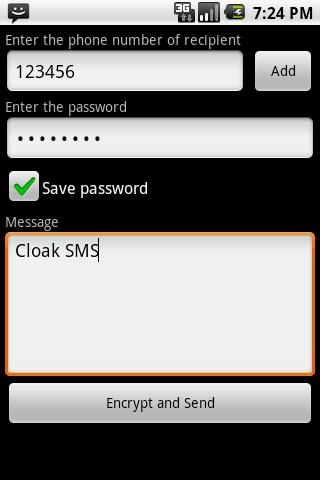
\includegraphics[scale=0.5]{images/cloaksms.jpg}
\caption{A screen capture of the application in use.}
\vspace{-10pt}
\label{fig:cloaksms}
\end{figure}

\subsection{RSA Cipher Cat}

RSA Cipher Cat is an application developed by Miasoft \cite{rsaciphercat}, which makes use of the RSA public-key encryption scheme. Figure \ref{fig:ciphercat} shows the two main screens of the application, one for encryption (\ref{fig:cat2}) and one for decryption (\ref{fig:cat1}). The disadvantage of this application is that it very basic, as it does not facilitate the sending of the messages, it only performs the actual encryption and decryption, using files given to the application by the user. It is then up to the user to send the encrypted message however they wish. Whilst it does not have the full features of the other applications, it is perfectly appropriate for this project, as it gives an insight into the current state of encrypted message sending applications and an example of cryptography in practice. The application is free to the public, but has a low user review rating of 1/5, submitted by a single user, whilst having between 500-1,000 installs. 

\begin{figure}
        \centering
        \begin{subfigure}[b]{0.45\textwidth}
                \centering
                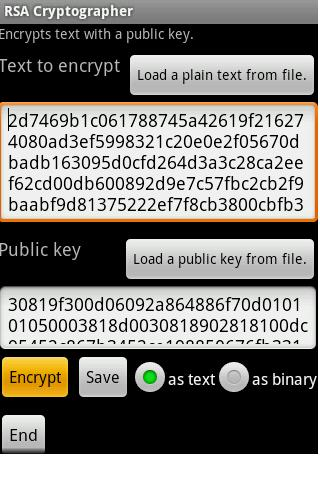
\includegraphics[width=\textwidth]{images/cat2.jpg}
                \caption{Encrypting a message}
                \label{fig:cat2}
        \end{subfigure}
	\begin{subfigure}[b]{0.45\textwidth}
                \centering
                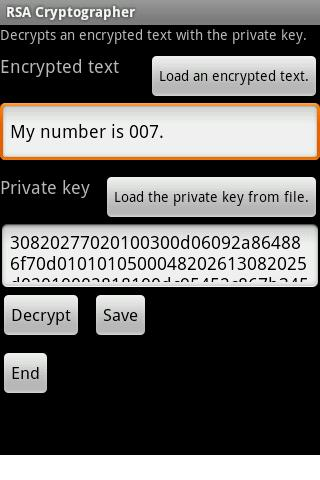
\includegraphics[width=\textwidth]{images/cat1.jpg}
                \caption{Decrypting a message}
                \label{fig:cat1}
        \end{subfigure}
        \caption{Application usage screen captures}\label{fig:ciphercat}
\end{figure}

\section{Cryptographic Techniques}

In this section of the report the cryptographic techniques, found as a result of the research completed, will be described and detailed in full, including examples and proofs where necessary. Research was completed using books by Wenbo Mao \cite{wenbomao} and William Stallings \cite{willstallings}. Any other texts or materials used within this research section will be individually referenced. 

It is important to firstly note that it was found that cryptographic schemes can be loosely sorted into two main categories; symmetric or asymmetric key algorithms. 

Symmetric key algorithms feature an encryption key that is identical (or easily computable from) the decryption key. This commonly means that decryption is similar or identical to running the encryption in verse.

Asymmetric key algorithms, on the other hand, operate using two keys called a key-pair; a publicly known key (public key) and a key kept in secret (private key) for each user. If user A wishes to send a message to user B, A encrypts the message using B's public key. The public and private key for each user are related in such a way that B can decrypt the message from A using B's private key. However, it is computationally infeasible for A (or any other user) to find B's private key from the corresponding public key.

Another way in which schemes can be categorised is by whether they operate on a block of input data (block ciphers) or a stream of input data (stream ciphers). As the categories are determined by the fundamental workings of the schemes, these categorisations are identical and present in all cryptographic related texts. 

\subsection{Advanced Encryption Standard}

The Advanced Encryption Standard (AES) algorithm is a symmetric-key block cipher and was chosen in 1997 by the United States' National Institute of Standards and Technology (NIST) to replace the previously used DES algorithm. AES typically uses a 128-bit block size and a key size of 128, 192 or 256. 

\subsubsection{Finite Field Arithmetic}

The internal functions of the AES cipher operate on 8-bit bytes, with the operations of addition, multiplication and division performed over the finite field GF($2^{8}$).
Arithmetic operations on integers are found in almost all encryption algorithms. If the arithmetic operation of division is required in the operation, then the arithmetic must be defined over a field, due to the fact that division requires that each non-zero element must have a multiplicative inverse. Furthermore, to increase implementation efficiency, it is required that integers fall into a given number of bits, with no wasted bit patterns; integers in the range 0 to $2^{n} - 1$, which fit into an $n$-bit word. However, the set of integers that follow this property, $Z_{2^{n}}$, using modular arithmetic, is not a field as, for example, 2 has no multiplicative inverse in the set. This means that there is no integer $b$, such that $2b$ mod $2^{n} = 1$. Therefore, the finite field containing $2^{n}$ elements, GF($2^{8}$), is used. Taking the set, S, of all polynomials of degree $n - 1$ or less with binary coefficients, every member is of the form
\[f(x) = a_{n-1}x^{n-1} + a_{n-2}x^{n-2} + ... + a_{1}x + a_{0} = \sum_{i=0}^{n-1}a_{i}x^{i}\] 
where each $a_{i}$ is either 0 or 1. Therefore, S consists of $`2^{n}$ different polynomials. For $n = 3$, the elements of S are:
\begin{center}
$
\begin{matrix}
  0 & x & x^{2} & x^{2} + x \\
  1 & x + 1 & x^{2} + 1 & x^{2} + x + 1 
 \end{matrix}
$
\end{center}
The ordinary rules of polynomial arithmetic using the basic rules of algebra is followed by arithmetic performed on elements of this set, with two alterations. Firstly, arithmetic performed on the coefficients is performed modulo 2. This is identical to the XOR operation. Secondly, if multiplication results in a polynomial of degree greater than $n - 1$, then the polynomial is divided by some irreducible polynomial $m(x)$ of degree $n$, with the remainder kept (polynomial is reduced modulo $m(x)$). For $f(x)$, the result is $r(x) = f(x)$ mod $m(x)$. $m(x)$ is described as irreducible if and only if $m(x)$ cannot be expressed as a product of two polynomials, both with degree lower than that of $m(x)$. These definitions result in S being a finite field.

Any polynomial in GF($2^{n}$) can be uniquely represented as ($a_{n-1}a_{n-2}...a_{0}$), its $n$ binary coefficients. Therefore, every polynomial in GF($2^{n}$) can be represented by an $n$-bit number. 

Taking the bitwise XOR of two terms is the equivalent of addition. 

Multiplication of an element in GF($2^{n}$) by 2 is made up of a left shift, followed by a conditional XOR with a constant. Repeated application of this rule can be used to achieve multiplications of higher orders.

For example, AES uses arithmetic in the finite field GF($2^{8}$) with $m(x) = x^{8} + x^{4} + x^{3} + x + 1$. Taking two elements of GF($2^{n}$)

\[ A = (a_{7}a_{6}...a_{1}a_{0}) \]
\[ B = (b_{7}b_{6}...b_{1}b_{0}) \]
\[ A + B = (c_{7}c_{6}...c_{1}c_{0})\]

where $c_{i} = a_{i} \oplus b_{i}$ and

\[
    \{02\} \bullet A = 
\begin{cases}
    (a_{6}...a_{1}a_{0}0) & \text{if } a_{7} = 0\\
    (a_{6}...a_{1}a_{0}0) \oplus (00011011) & \text{if } a_{7} = 1
\end{cases}
\]

\subsubsection{Structure}

The AES cipher takes an input plaintext in blocks of 128 bits (16 bytes). The key used can have a length of 128, 192 or 256 bits (16,24 or 32 bytes). The input block (and the chosen key) can be depicted as a 4x4 matrix of bytes. This input block is copied into a State array, which is the array that is operated upon during for the duration of the algorithm. The resulting State array is finally copied into an output matrix once the transformations have been completed. The algorithm operates by performing a number of transformations on the input plaintext block. The number of rounds of transformations is determined by the size of the key chosen. 

\begin{description}
 \item[16 byte key] - 10 rounds
 \item[24 byte key] - 12 rounds
 \item[32 byte key] - 14 rounds
\end{description}

The key chosen for the encryption scheme is initially expanded, using the original 4x4 byte key, to provide a 4x4 byte Round Key for each round. This means that the initial 16 byte key (4 words) is expanded to 176 bytes (44 words). This provides 11, 4 word (4x4 byte) rounds keys. As the original key is 16 bytes, 10 rounds of transformations will be applied, plus an initial usage of a Round Key, hence 11 Round Keys are required.

The structure of the AES cipher is as follows:

\begin{enumerate}
 \item Round 0 
 \begin{enumerate}
  \item AddRoundKey(State,RoundKey) 
 \end{enumerate}
 \item Round 1 to N-1
 \begin{enumerate}
  \item SubBytes(State) 
  \item ShiftRows(State) 
  \item MixColumns(State)
  \item AddRoundKey(State,RoundKey) 
 \end{enumerate}
 \item Final Round
 \begin{enumerate}
  \item SubBytes(State) 
  \item ShiftRows(State)
  \item AddRoundKey(State,RoundKey) 
 \end{enumerate}
\end{enumerate}

Before describing each transformation in detail, some interesting and important points regarding the structure of the AES algorithm shall be made. Firstly, AES does not follow a typical Feistel structure, where half of the data block is used to modify the other half and then the halves are swapped. Instead, the entire data block is processed as a single matrix during each round. 

Also, the AddRoundKey stage is the only stage that makes use of the key. Therefore, the cipher must begin and end with an AddRoundKey stage, as any other stage applied before or after this would be reversible without knowledge of the key, which would add no security. The AddRoundKey stage is, by itself, not formidable. The other three stages create confusion, diffusion and non-linearity, enabling the algorithm to be described as an alternation of the XOR encryption (AddRoundKey) of a block and the scrambling of the block (other three stages). This creates an efficient and highly secure scheme. 

Lastly, the final round of encryption (and decryption) consists of only three stages. This is as a result of the structure of AES and is required for the cipher to be reversible. 

\subsubsection{Functions}

Each function will now be taken and described individually. 

\paragraph{Sub-bytes}

The sub-bytes transformation consists of a non-linear substitution of each byte of the input State. The following equation (using the rules of arithmetic defined previously) is used to transform the non-zero input byte $x \in$ GF($2^{8}$): 

\begin{equation}
 y = Ax^{-1} + b
\label{eq:subbyteeq}
\end{equation}

where
$
A = 
\begin{pmatrix}
  1 & 0 & 0 & 0 & 1 & 1 & 1 & 1 \\
  1 & 1 & 0 & 0 & 0 & 1 & 1 & 1 \\
  1 & 1 & 1 & 0 & 0 & 0 & 1 & 1 \\
  1 & 1 & 1 & 1 & 0 & 0 & 0 & 1 \\
  1 & 1 & 1 & 1 & 1 & 0 & 0 & 0 \\
  0 & 1 & 1 & 1 & 1 & 1 & 0 & 0 \\
  0 & 0 & 1 & 1 & 1 & 1 & 1 & 0 \\
  0 & 0 & 0 & 1 & 1 & 1 & 1 & 1
 \end{pmatrix}
$
and
$ 
b = 
 \begin{pmatrix}
   1 \\ 1 \\ 0 \\ 0 \\ 0 \\ 1 \\ 1 \\ 0 
 \end{pmatrix}
$

If $x$ is the zero byte, then $y = b$ is the result. 

More commonly, the transformation in (\ref{eq:subbyteeq}) is used to generate a simple lookup table called an S-box, shown in Figure \ref{fig:sbox}. The S-box is a permutation of all possible 256 8-bit values. Each byte of the input State can be substituted with the new value by using the leftmost 4 bits of the byte as the row value and the rightmost 4 bits as the column value. Using these values as indexes to the new value from the S-box, resulting in a new 8 bit output value. For example, the hexidecimal value $\{89\}$ references row 8 and column 9 of the S-box and will thus be mapped to $\{A7\}$. The constant in (\ref{eq:subbyteeq}) has been chosen so that no fixed points exist within the S-box (S-box$(a) \neq a $). Furthermore, no 'opposite' fixed points exist (S-box$(a) \neq \overline{a} $), where $\overline{a}$ is the bitwise complement of $a$. 

\begin{figure}[htb]
\centering
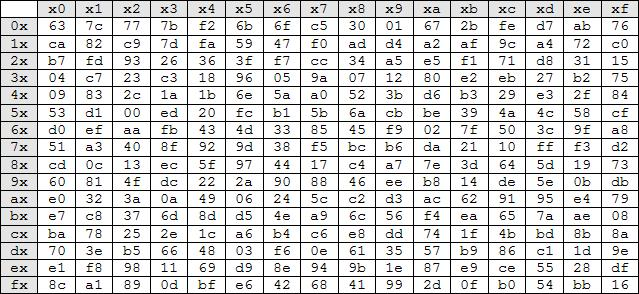
\includegraphics[scale=0.5]{images/sbox.jpg}
\caption{AES S-box}
\label{fig:sbox}
\end{figure}

The non-linearity of the transformation in (\ref{eq:subbyteeq}) is a result of the inversion $x^{-1}$ (multiplicative inverse) only. Since the rows of $A$ are linearly independent in GF($2^{8}$), the transformation (\ref{eq:subbyteeq}) and hence the function Sub-Bytes, is invertible. The inverse S-box can be generated in the same way using the inverse of (\ref{eq:subbyteeq}).

\paragraph{ShiftRows}

The operation ShiftRows is described as a transposition cipher, only the positions of the elements are rearranged not their identities. For elements in the $i$th ro ($i = 0 1 2 3)$, the rearrangment is a cyclic shift by $4 - i$ positions. This is shown in Figure \ref{fig:shiftrows}.

\begin{figure}[htb]
\centering
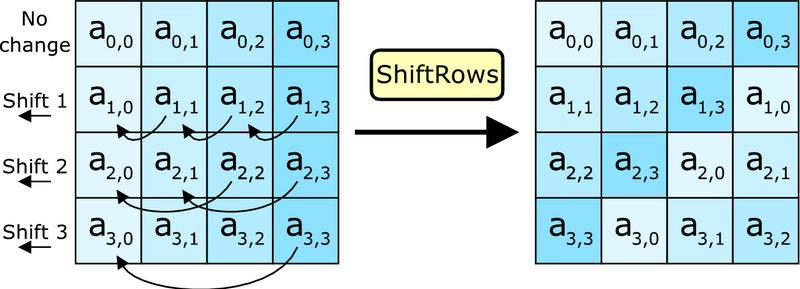
\includegraphics[scale=0.3]{images/shiftrows.jpg}
\caption{ShiftRows transformation}
\label{fig:shiftrows}
\end{figure}

It can be clearly seen that the result of this transformation is that the elements (4 bytes) of each original column are spread out to four different columns in the output, which is the rationale behind this operation. As only the positions are changed or elements in the State, the transformation is clearly invertible. 

\paragraph{MixColumns}

The MixColumns function operates on each column individually, with each byte of the column mapped into a new value that is determined by the value of all four bytes in that column. The transformation can be defined by a matrix multiplication on the input state shown in Figure \ref{fig:mixcols1} taken from \cite{aesmixcols}.

\begin{figure}[htb]
\centering
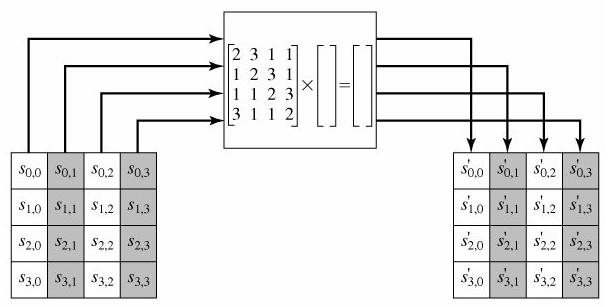
\includegraphics[scale=0.6]{images/mixcols1.jpg}
\caption{MixColumns transformation}
\label{fig:mixcols1}
\end{figure}

All additions and multiplications are performed in GF($2^{8}$). The transformation on a single column of the input State can be seen in Figure \ref{fig:mixcols2} (\cite{aesmixcolssecond}).

\begin{figure}[htb]
\centering
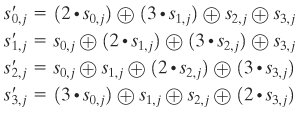
\includegraphics[scale=0.7]{images/mixcols2.jpg}
\caption{MixColumns transformation on a single column}
\label{fig:mixcols2}
\end{figure}

The following is an example of the MixColumns transformation:

\begin{figure}[htb]
\centering
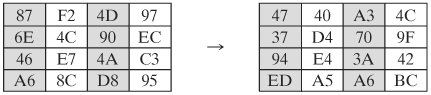
\includegraphics[scale=0.7]{images/mixcolsexample.jpg}
\caption{MixColumns transformation example}
\label{fig:mixcolsexample}
\end{figure}

Recalling the rules for arithmetic in GF($2^{8}$) presented previously, the first resulting element of the example can be verified. 

\begin{center}

$ (\{02\}\bullet \{87\}) \oplus (\{03\} \bullet \{6$E$\}) \oplus (\{46\}) \oplus (\{$A$6\}) = (\{47\}) $
\end{center}
\begin{center}
$ (\{02\}\bullet \{87\}) = (00001110) \oplus (00011011) = (00010101) $
$ (\{03\} \bullet \{6$E$\}) = (\{6$E$\} \oplus (\{02\} \bullet \{6$E$\}) = (01101110) \oplus (11011100) = (10110010) $
\end{center}

Then 

\begin{center}
 $ (\{02\}\bullet \{87\}) \oplus (\{03\} \bullet \{6$E$\}) \oplus (\{46\}) \oplus (\{$A$6\}) $
\end{center}

is equal to

\begin{center}
 $ (00010101) \oplus (10110010) \oplus (01000110) \oplus (110100110) = (01000111) = (\{47\})$
\end{center}

The other equations can be verified in a similar way. The inverse of this operation can be computed using the following matrix multiplication:

\begin{figure}[htb]
\centering
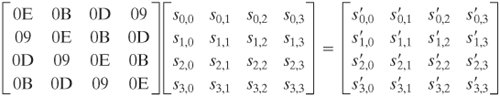
\includegraphics[scale=0.7]{images/invmixcols.jpg}
\caption{The inverse MixColumns operation}
\label{fig:invmixcols}
\end{figure}

The coefficients chosen for the matrix in Figure \ref{fig:mixcols1} ensure a sufficient mixing among the bytes of each column. A combination of the MixColumns and ShiftRows operations ensures that after a few rounds, all the output bits depend upon all of the input bits. 

\paragraph{AddRoundKey}
The AddRoundKey operation is the final transformation for each round. The 128 bits of the input State are bitwise XORed (addition in GF($2^{8}$)) with the 128 bits of the current round key. The operation is viewed as a columnwise operation between the 4 bytes of the input State and one word of the round key and is therefore a byte-level operation. Figure \ref{fig:addroundkey1} shows an example of the AddRoundKey operation, where the first matrix is the State and the second is the Round Key. 

\begin{figure}[htb]
\centering
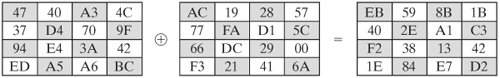
\includegraphics[scale=0.7]{images/addroundkey1.jpg}
\caption{An example of the AddRoundKey operation}
\label{fig:addroundkey1}
\end{figure}

The inverse of this operation is identical to this due to the fact that the XOR operation is its own inverse. The AddRoundKey transformation affects every bit of the input State and is as simple as possible. However, security is ensured through the complexity of the round key expansion and the complexity of the other stages of AES. 

\subsubsection{Key Expansion}

As mentioned previously, key expansion is required to expand the key into a number of Round Keys, one for each round of the AES algorithm. For example, a four-word (16 byte) key is expanded into an array of 44 words (176 bytes), providing a four-word round key for each of the 10 rounds plus the initial AddRoundKey. 

To begin, the four-word key is copied into the first four words of the expanded key. The remaining words of the expanded key are generated and copied four words at a time. Each new word $w[i]$ is calculated depending on the preceding word, $w[i-4]$ and the word four positions before it, $w[i-4]$. 

For three of the four cases, the two words are combined using the XOR operation. However, if the words position in the array is a multiple of 4, a more complex function is used. Figure \ref{fig:keyexp1} shows the key expansion for the first eight words of the expanded key (two round keys). The function g represents the complex function used for a word in a position that is a multiple of 4.

\begin{figure}[htb]
\centering
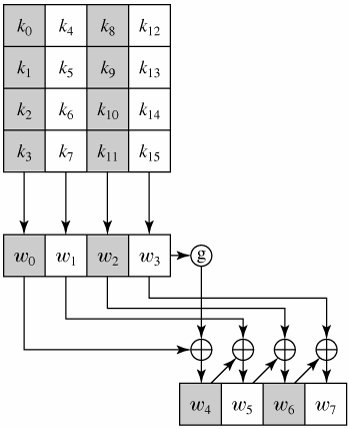
\includegraphics[scale=0.7]{images/keyexp1.jpg}
\caption{Basic key expansion diagram}
\label{fig:keyexp1}
\end{figure}

The function g is comprised of the following:

\begin{enumerate}
 \item \begin{description}
  \item[RotWord] One-byte circular left shift on a word. This means input word [B$_{0}$,B$_{1}$,B$_{2}$,B$_{3}$] becomes [B$_{1}$,B$_{2}$,B$_{3}$,B$_{0}$].
 \end{description}
 \item \begin{description}
  \item[SubWord] Byte substitution on each byte of the input word, using the S-box (Figure \ref{fig:sbox}).
 \end{description}
 \item \begin{description}
  \item[Rcon] The output from steps 1 and 2 are XORed with a round constant, Rcon[j]. 
 \end{description}
\end{enumerate}

The effect of an XOR between the round constant and a word is to only perform an XOR on the left-most byte of the word, due to the fact that the round constantt is a word in which the three right-most bytes are always 0. Each round uses a different round constant and is defined as Rcon[j] = (RC[j],0,0,0) with RC[1] = 1, RC[j] = 2 $\bullet$ RC[j-1], with multiplication defined over the field GF($2^{8}$)). In hexidecimal, the values of RC[j] are found in Table \ref{tab:rcj}.

\begin{table}[h]
\begin{center}
    \begin{tabular}{| l | l | l | l | l | l | l | l | l | l | l |}
    \hline
    j & 1 & 2 & 3 & 4 & 5 & 6 & 7 & 8 & 9 & 10\\ \hline
    RC[j] & 01 & 02 & 04 & 08 & 10 & 20 & 40 & 80 & 1B & 36\\
    \hline
    \end{tabular}
   \caption{Hexidecimal RC[j] values}
    \label{tab:rcj}
\end{center}
\end{table} 

\begin{figure}[htb]
\centering
\lstinputlisting[basicstyle=\scriptsize, language=Java]{documents/keyexpcode.java}
\caption{Key Expansion }
\label{fig:keyexpcode}
\end{figure}

Figure \ref{fig:keyexpcode} shows a Java based pseudo-code representation of the key expansion algorithm.

The design and inclusion of a round key means that:
\begin{itemize}
 \item If part of the cipher key or round key is known, then the calculation of other round key bits is not possible.
 \item Symmetry or similarity between the ways in which round keys are generated in different rounds is eliminated (use of a round-dependent constant)
 \item Each key bit affects many of the future round key bits (diffusion of the cipher key).
 \item Only enough non-linearity is used to ensure that the full determination of round key differences from cipher key differences is prohibited. 
\end{itemize}

\subsubsection{Decryption}

%stallings book, bottom yellow sticky

Decryption of the AES cipher algorithm essentially involves running the encryption scheme 'backwards' or applying the encryption scheme again but in reverse, using the inverse operations of those operations used for encryption. 

As shown previously, each stage is clearly reversible. SubBytes, ShiftRows and MixColumns each have an associated inverse function. With AddRoundKey, the inverse is calculated by XORing the same round key to the block, due to the fact that A $\oplus$ B $\oplus$ B = A. Now that it is established that all four operations are reversible, it can be easily verified that the correct plaintext is recovered through decryption. 

Figure \ref{fig:decrypt1} shows the comparison between encryption and decryption. At each horizontally equal point, the value of the State is the same for both encryption and decryption. In order for the structure of the cipher to be reversible, both the encryption and decryption end with a final round of three stages. 

\begin{figure}[htb]
\centering
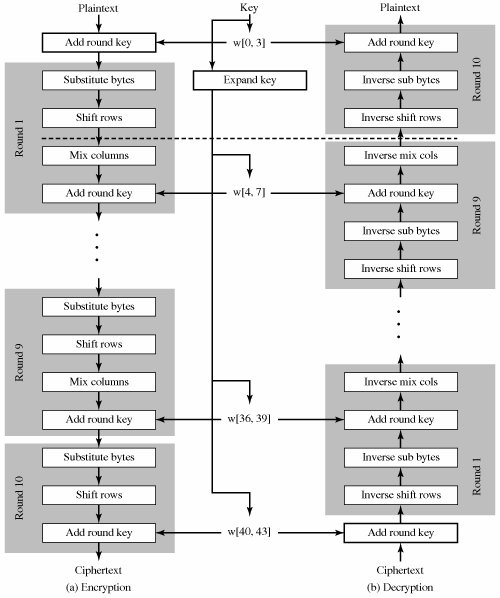
\includegraphics[scale=0.7]{images/decrypt1.jpg}
\caption{AES Encryption and Decryption}
\label{fig:decrypt1}
\end{figure}

\subsubsection{Example}

Instead of presenting a formal example of the AES cipher, the reader is directed to the example by William Stallings on page 193 of \cite{willstallings}. A formal example is not displayed due to the complexity of computing the calculations required by hand and the fact that an example would add no benefit to this section of the report, as an understanding of this scheme has already been shown through the explanation of its operation. 

\subsubsection{Implementation}

%other bottom yellow sticky

As encryption schemes are used primarily in computer based systems, consideration must be made about how the functions that make up the cipher are implemented. Different implementations of a similar function made lead to a suboptimal or insecure system. It can be seen from the description of the AES cipher that the internal functions are fairly simple and operate in small algebraic spaces. Because of this, implementations of the operations can be done with extremely good efficiency. AddRoundKey is a bytewise XOR operation and ShiftRows is a simple byte-shifting operation, so can be implemented with good efficiency on any size processor. SubBytes and MixColumns, however, have non-trivial algebraic operations and therefore should be looked at in more detail to find faster implementation methods. 

SubBytes, as shown in the description of the operation, can be completed using a table lookup method, rather than calculating individual values each time. The table of $2^{8} = 256$ pairs of bytes can be generated once and used forever (hard-coded into either hardware or software). The table lookup method is not only efficient, but also prevents a timing analysis attack, which is based upon a malicious user observing the operation time difference for different data which may suggest whether an operation is performed on bit 0 or bit 1. Inversion can clearly be completed using the inversion table. Therefore, SubBytes can be implemented using two, 256 byte, tables. 

MixColumns can also be improved using a table lookup method. All multiplications (within the field) required to complete MixColumns, are of the form $z = x \cdotp y$ where $x \in \{01,02,03\}$ and $y \in $GF($2^{8}$) (see Figure \ref{fig:mixcols2}. As the byte $01$ is simply the multiplicative identity in the field ($01 \cdotp y = y$), an implementation of this multiplication table only requires $2$ x $256 = 512$ entries. Using this implementation technique not only increases operation speed, but also decreases the risk of a timing analysis attack. 

\subsubsection{Summary}

To conclude the study of the AES cipher, a short summary:

\begin{itemize}
 \item The cipher contains a number of rounds of operations, the number of which is determined by the key size.
 \item Key sizes normally take the values: 128-bits (10 rounds), 192-bits (12 rounds) and 256 (14 rounds).
 \item The key is expanded to provide a 4-word round key for each round.
 \item The internal functions of the AES algorithm are:
    \begin{itemize}
     \item SubBytes: non-linear substitution.
     \item ShiftRows and MixColumns: mixture of byte positions of the input State.
     \item AddRoundKey: secret randomness to the message distribution.
    \end{itemize}

\end{itemize}

\subsection{Rivest-Shamir-Aldeman Algorithm}

Published in 1978, the Rivest-Shamir-Aldeman (RSA) scheme \cite{rsa} is one of the most widely accepted and implemented approaches to public-key encryption. The RSA algorithm is based upon the difficulty of factoring large integers. It acts as a block cipher in which for some n, the ciphertext and plaintext are integers between 0 and n. Typically, n is less than 1024 bits or 309 decimal digits (n is less than $2^{1024}$). Hence, the actual message is split into plaintext blocks using a chosen encoding method, with each block encrypted and decrypted separately. 

The operation of the RSA encryption scheme has three parts: Key generation, Encryption and Decryption. The description of this scheme uses the common placeholder names of Alice and Bob inkeeping with tradition set out by Bruce Schneier \cite{bruceschneier}.

\subsubsection{Background}

The RSA algorithm utilises mathematical techniques and results which will be presented now, before the main algorithm is described.

\paragraph{Euler's Totient Function}

Written as $\phi(n)$, Euler's totient function is defined as the number of positive integers less than $n$ and relatively prime (commonly divisible by only 1) to $n$. By convention, $\phi(1) = 1$. 

Clearly, for a prime number $p$, $\phi(p) = p - 1$, as all positive integers from 1 to $p - 1$ are relatively prime to $p$. Taking two prime numbers $p$ and $q$ with $p \neq q$, it can be shown that for $n = pq$

\[\phi(n) = \phi(pq) = \phi(p) \times \phi(q) = (p - 1) \times (q - 1) \]

To show that $\phi(n) = \phi(p) \times \phi(q)$, consider the set of positive integers less than $n$, $\{1, ..., (pq - 1)\}$. The integers that are not relatively prime to n in this set are the sets $\{p,2p, ..., (q - 1)p\}$ and $\{q,2q, ..., (p - 1)q\}$ (containing $(q - 1)$ and $(p - 1)$ elements respectively). Therefore:

\begin{center}
$\begin{array}{lcl} \phi(n) & = & (pq - 1) - [(q - 1) + (p - 1)] \\  
			    & = & pq - (p + q) + 1 \\
			    & = & (p - 1) \times (q - 1) \\
			    & = & \phi(p) \times \phi(q) 
\end{array}$
\end{center}

As an example:

\[ \phi(21) = \phi(3) \times \phi(7) = (3 - 1) \times (7 - 1) = 2 \times 6 = 12 \]
where the 12 integers are $\{1,2,4,5,8,10,11,13,16,17,19,20\}$.

\subsubsection{Description}

The RSA algorithm is an example of an asymmetric key algorithm, in which a public key and a private key are utilised. The public key is shared and known with everyone and used in the encryption process. The messages encrypted with the public key can only be decrypted using the matching private key. For some plaintext block M and ciphertext block C, encryption and decryption are of the following form: 

\[ C = M^{e} \bmod(n) \]
\[ M = C^{d} \bmod(n) = (M^{e})^{d} \bmod(n) = M^{ed} \bmod(n)\]

The keys for this algorithm are therefore; the private key PR = $\{d,n\}$ and the public key PU = $\{e,n\}$. For this algorithm to be securely used for public-key encryption, the following requirements must be satisfied.
\begin{enumerate}
  \item Values of e, d and n can be found such that $ M^{ed} \bmod(n) = M $ for all $ M < n $.
  \item $ M^{e} \bmod(n) $ and $ C^{d} \bmod(n) $ are relatively easy to compute, for all values of $ M < n $.
  \item It is infeasible to determine d given e and n.
\end{enumerate}

The first required will be considered now, with the other requirements being described later in this section. The relationship that needs to be satisfied is $ M^{ed} \bmod(n) = M $, which holds if $e$ and $d$ are multiplicative inverses modulo $\phi(n)$, where $\phi(n)$ is the Euler totient function as described previously. The relationship between $e$ and $d$ can be expressed as:

\[ ed \bmod \phi(n) = 1 \]
which is equivalent to
\[ ed = 1 \bmod \phi(n) \]
\[ d = e^{-1} \bmod \phi(n) \]

Therefore, $e$ and $d$ are multiplicative inverses $\bmod \phi(n)$, which is only true if $d$ and $e$ are relatively prime to $\phi(n)$. This satisfies the first requirement for the RSA algorithm (a proof of which will be presented towards the end of this section). The stages of the RSA algorithm can no be presented. 

\paragraph{Key Generation}

The following process is used to generate the required keys:

\begin{enumerate}
  \item Choose two distinct prime numbers $p$ and $q$.
  \begin{itemize}
    \item These are chosen at random and kept private.
  \end{itemize}
  
  \item Calculate $ n=pq $.
  
  \item Calculate $ \phi(n)=(p-1)(q-1) $
  
  \item Choose e such that $ 1 < e < \phi (n) $ and $e$ and $ \phi(n) $ are coprime
  
  \item Determine d as $ d = e^{-1} \bmod \phi (n) $. Here d is the multiplicative inverse of $ e \bmod \phi (n) $.
  
\end{enumerate}

Therefore the private key consists of [$d,n$] and the public key consists of [$e,n$]. The private key must be kept secret whereas the public key can be shared. $p$, $q$ and $ \phi(n) $ must also be kept secret as they were used to calculate $d$. This is how RSA can be described as being based on the difficulty of factoring large numbers. If it where computationally easy to find the prime factors of a number, in this case $n$, then using the factors $p$ and $q$, $\phi(n)$ could be easily calculated. Combining this with the knowledge of the public value $e$ would allow the calculation of $d$, breaking the encryption scheme. Therefore, until a computationally efficient way of finding the prime factors of a large number is discovered, the RSA algorithm remains secure. 


\paragraph{Encryption}

Bob wants to send a message M to Alice. Alice sends Bob her public key $ K_{a} \, = {e,n} $ and keeps her private key secret. Bob computes the ciphertext C corresponding to
\[ C = M^{e} \bmod(n) \]
Bob then sends C to Alice.

\paragraph{Decryption}

Alice receives ciphertext C from Bob. She can recover the message M from C using her private key by computing
\[ M = C^{d} \bmod(n) \]

\textit{Note: M is an integer between 0 and $n$, so Alice and Bob must agree upon a method to turn their message text into plaintext blocks (integers) and back again, for example a = 00, A = 26 etc.}

\subsubsection{Example}

To aid in the explanation of this algorithm, an original basic example will be presented:

\begin{enumerate}
 \item Select two prime numbers, $p=13$ and $q=11$.
 \item Calculate $n=pq=13\times11=143$.
 \item Calculate $\phi(n)=(p-1)(q-1)=12\times10 = 120$.
 \item Select $e$, relatively prime to $\phi(n)=120$ and less than $\phi(n)$; $e=7$.
 \item Determine $d$ such that $de \equiv 1 \bmod(120)$ and $d < 160$. $d = 103$ as $103 \times 7 = 721 = (6 \times 120) + 1$.
\end{enumerate}

This results in PU $= \{7,143\}$ and PR $= \{103,143\}$. With a plaintext input of $M = 44$, encryption (and decryption) are as follows:

\[ C = 44^{7} \bmod(143) = 99 \]
\[ M = 99^{103} \bmod(143) = 44 \]

\subsubsection{Implementation}

As with the AES cipher, the computational aspects of the RSA algorithm need to be considered. The main three issues that require consideration are presented bellow.

\paragraph{Exponentiation in Modular Arithmetic}

As both encryption and decryption require raising an integer to an integer power $\bmod(n)$, processes in which to improve the implemented efficiency should be developed. If the exponentiation is calculated and the result is then reduced modulo $n$, the intermediate values would be colossal. However, a property of modular arithmetic can be utilised:

\[ [(a\bmod n)\times(b \bmod n)] \bmod n = (a \times b) \bmod n \]

which makes calculations much more practical. 

The efficiency of the exponentiation should also be considered. This is because in RSA, the exponents are potentially very large. As an example to show how efficiency can be increased, consider $x^{8}$, which can be computed as;

\[ x^{8} = x \times x \times x \times x \times x \times x \times x \times x \]

or by repeatedly taking the square of the previous partial result forming ($x^2,x^4,x^8$), a less computationally expensive calculation. This can be extended to calculations like $x^{11}$, where $x^{11} = x^{1+2+8}$. In this case

\[ x^{11} = [(x \bmod n) \times (x^2 \bmod n) \times (x^8 \bmod n)] \bmod n \]

\paragraph{Public Key Operation}

Through a specific choice of $e$, the speed of operation of the RSA algorithm utilising the public key can be greatly increased. Most commonly, values for e are chosen as $65537 (2^{16} + 1), 3$ or $17$. This is due to the fact that each of the three choices contain only two 1 bits, which minimises the number of multiplications required to perform the exponentiation. Very low values of $e$ ($e = 3$), however, decrease the security of RSA, so larger values, primarily $65537$, are the most popular. 

\paragraph{Key Generation}

Because $n=pq$ will be public known to any adversary, the prime numbers $p$ and $q$ must be sufficiently large to prevent their discovery by exhaustive methods. On the other hand, the method used for generating these large numbers must be reasonably efficient. Unfortunately, at present, there are no useful methods for generating arbitrarily large prime numbers, so other techniques must be used to tackle the problem. One procedure is to pick a random odd number of the desired magnitude, tests its primality and repeat if it is not prime. Whilst this may seem to increase the inefficiency of the algorithm, it only needs to be completed relatively infrequently, when two users wish to communicate for the first time. Therefore, an vast increase in security is chosen over an initial, slightly large, time cost. However, using the prime number theorem from number theory\footnotemark\label{fnm:1} \footnotetext{The number of primes near N are spaced on average one every (ln$N$) integers.\label{fnt:1}}and the fact that all even numbers can be immediately rejected, the number of tests required would be of the order of ln($N$). For example, if a prime on the order of magnitude of $2^{200}$ is required, then about ln($2^{200})$\textfractionsolidus $2 = 70$ tests would be needed to find a prime. 

\subsubsection{Proof of the RSA Algorithm}

The main elements of the RSA algorithm can be expressed in the following equation:

\[ M^{ed} \bmod n = M \]

which holds if $e$ and $d$ are multiplicative inverses modulo $\phi(n)$. The relationship between $e$ and $d$ can be expressed as:

\[ ed \bmod \phi(n) = 1 \]

or that there is an integer $k$ such that

\[ ed = k\phi(n) + 1 \]

Thus, it will be shown in this section that the following holds

\begin{equation}
 M^{k\phi(n) + 1} \bmod n = M^{k(p-1)(q-1) + 1} \bmod n = M
\label{eq:proof}
\end{equation}

Three other results that are required for the proof of Equation \ref{eq:proof} are

\[ [(a\bmod n)\times(b \bmod n)] \bmod n = (a \times b) \bmod n \]
\[ [(a\bmod n) - (b \bmod n)] \bmod n = (a - b) \bmod n \]
and if integers $a$ and $n$ are relatively prime, then
\[a^{\phi(n)} \bmod n = 1 \]

This last result is named Euler's theorem. 

\subparagraph{Proof}

First we show that $M^{k(p-1)(q-1) + 1} \bmod p = M \bmod p$. Here, there are two cases to consider:

\begin{description}
 \item[$M$ and $p$ are not relatively prime] ($p$ divides $M$) This means that $M \bmod p = 0$ and $M^{k(p-1)(q-1) + 1} \bmod p = 0$ and so they are equal. 
 \item[$M$ and $p$ are relatively prime] By Euler's theorem $M^{\phi(p)} \bmod p = 1$.
\end{description}

It follows that

\begin{center}
$\begin{array}{lcl} M^{k(p-1)(q-1) + 1} \bmod p & = & M[M^{k(p-1)(q-1)1}] \bmod p  \\  
						& = & M[(M^{(p-1)})^{k(q-1)}] \\
						& = & M[(M^{\phi(p)})^{k(q-1)}]  \\
						& = & (M \bmod p) \times [(M^{\phi(p)}) \bmod p]^{k(q-1)} \\
						& = & (M \bmod p) \times (1)^{k(q-1)} \\
						& = & (M \bmod p) 
\end{array}$
\end{center}

Which shows that 

\[ [M^{k(p-1)(q-1) + 1} - M]\bmod p = [M^{k(p-1)(q-1) + 1} \bmod p] - [M \bmod p] = 0 \]

Thus, $p$ divides $[M^{k(p-1)(q-1) + 1} - M]$. The same reasoning can be used to show the $q$ divides $[M^{k(p-1)(q-1) + 1} - M]$. Because $p$ and $q$ are distinct primes, there must exist an integer $r$ that satisfies 

\[ [M^{k(p-1)(q-1) + 1} - M] = (pq)r = nr \]

Therefore, $n$ divides $[M^{k(p-1)(q-1) + 1} - M]$, and so

\[ M^{k\phi(n) + 1} \bmod n = M^{k(p-1)(q-1) + 1} \bmod n = M \]

\subsubsection{Summary}

The RSA algorithm is a public-key scheme, based upon the difficulty of factoring large numbers. Figure \ref{fig:rsasum} summarises the operation of the algorithm.

\begin{figure}[htb]
\centering
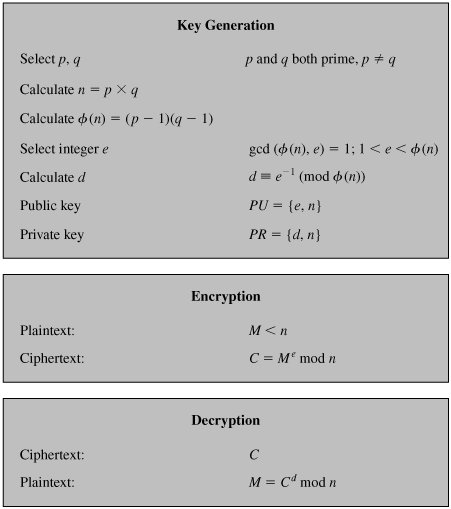
\includegraphics[scale=0.7]{images/rsasum.jpg}
\caption{Summary of the RSA algorithm}
\label{fig:rsasum}
\end{figure}

\subsection{Elliptic Curve Cryptography}

\subsubsection{Introduction}

Elliptic Curve Cryptography (ECC) is another approach to public-key cryptography (asymmetric key algorithm) but is based on the algebraic structure of elliptic curves over finite fields. The assumption that finding the discrete logarithm of a random elliptic curve element, with respect to a publicly known base point, is infeasible is the basis for the elliptic curve cryptographic scheme.

As with RSA, the ECC scheme is made up of three parts; key generation, encryption and decryption.

\subsubsection{Background}

This section will provide the background concepts and mathematical foundations on which ECC is based.

\paragraph{Abelian Groups}

An abelian group $G$, is a set of elements with a binary operation $\bullet$, that associates to each ordered pair $(a,b)$ of elements in $G$ an element $(a \bullet b)$ in $G$, such that the following axioms are obeyed;

\begin{description}
 \item[(A1) Closure:] If $a , b \in G$ then $a \bullet b \in G$.
 \item[(A2) Associative:] $a \bullet (b \bullet c) = (a \bullet b) \bullet c \:\: \forall a,b,c \in G$.
 \item[(A3) Identity Element:] $\exists e \in G$ such that $a \bullet e = e \bullet a = a \;\; \forall a \in G$
 \item[(A4) Inverse Element:] For each $a \in G \; \exists a' \in G$ such that $a \bullet a' = a' \bullet a = e$.
 \item[(A5) Commutative:] $a \bullet b = b \bullet a \; \forall a,b \in G$. 
\end{description}

Note that the operator $\bullet$ is generic and can reger to an mathematical operation. 

\paragraph{Elliptic Curves over Real Numbers}

Elliptic curves are named as such, not becase they are ellipses, but because they are described by cubic equations, similar to those used for calculating ellipse circumferences. The purposes of cryptograpy, elliptic curves are cubic equations of the form:

\begin{equation}
y^2 = x^3 + ax + b 
\label{eq:mainecceq}
\end{equation}

Included in the description of an elliptic curve is the 'point at infinity' or the 'zero point' denoted $O$. The equation

\[y = \sqrt{x^3 + ax + b}\]

is used to plot such a curve, which consists of a positive and negative value of $y$ for each $x$ value and so is symmetric about $y=0$. 

Consider the set of points $E(a,b)$ consisting of all the points $(x,y)$ that satisfy Equation \ref{eq:mainecceq} together with element $O$. Varying the pair $(a,b)$ results in a different set $E(a,b)$ and thus a different elliptic curve. Figure \ref{fig:eccbaseexample} shows two examples of elliptic curves. 

\begin{figure}[htb]
\centering
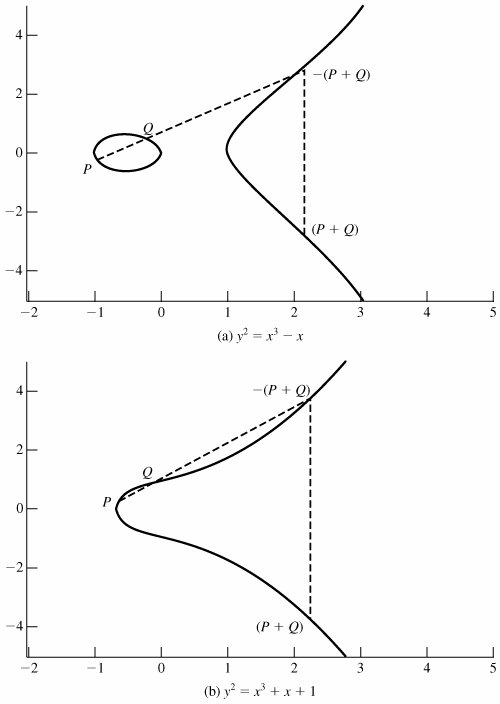
\includegraphics[scale=0.7]{images/eccbaseexample.jpg}
\caption{Examples of Elliptic Curves}
\label{fig:eccbaseexample}
\end{figure}

A group can be defined based on the set $E(a,b)$ for specific values of $a$ and $b$ in Equation \ref{eq:mainecceq}, provided the condition

\begin{equation}
 4a^3 + 27b^2 \neq 0
\label{eq:abrelecc}
\end{equation}

is met. To define the group, the operation called addition (denoted by $+$), for the set $E(a,b)$ (where $a$ and $b$ satisfy Equation \ref{eq:abrelecc}), needs to be defined. In geometric terms, the rules for addition can be stated as: If three points on an elliptic curve lie on a straight line, their sum is $O$. From this, the rules of addition over an elliptic curve can be defined. 

\begin{enumerate}
 \item The identity element is $O$, thus $O = -O$ and $\forall P$ on the curve $P + O = P$. The following assumes $P \neq O$ and $Q \neq O$.
 \item If $P = (x,y)$ then $-P = (x,-y)$. Thus $P + (-P) = P - P = O$
 \item The addition of two points $P$ and $Q$, with different $x$ coordinates, is found on the plotted curve by drawing a straight line between them and finding the third point of intersection $R$. If the line is a tangent to the curve at $P$ or $Q$ then $R = P$ or $R = Q$. To form a group structure, addition needs to be defined on these three points: $P + Q = -R$, where $P + Q$ is the mirror image (with resepect to the $x$ axis) of the third point of intersection, shown in Figure \ref{fig:eccbaseexample}. 
 \item Geometrically, the preceding item also applies to the points $P$ and $-P$, showing that $P + (-P) = O$, which is consistent with item (2).
 \item Drawing the tangent line at point $Q$ and finding the other point of intersection $S$, allows the calculation of $2Q$, where $Q + Q = 2Q = -S$.
\end{enumerate}

With these set of rules, $E(a,b)$ is an abelian group. 

The calculation of additions over elliptic curves can now be presented. For two distinct points, $P = (x_{P},y_{P})$ and $Q = (x_{Q},y_{Q})$, where $P \neq -Q$, the slope of the line $l$ that joins them is $\Delta = (y_{Q} - y_{P})$\textfractionsolidus$(x_{Q} - x_{P})$. There is exactly one other point where $l$ intersects the elliptic curve; $-(P + Q)$. After some algebraic manipulation, the sum $R = P + Q$ can be expressed as:

\begin{equation}
  x_{R} = \Delta^{2} - x_{P} - x_{Q} 
  \label{eq:eccbaseadd1}
\end{equation}

\begin{equation}
  y_{R} = -y_{P} + \Delta(x_{P} - x_{R})
  \label{eq:eccbaseadd2}
\end{equation}

A point also needs to be added to itself: $P + P = 2P = R$. When $y_{P} \neq 0$, the expressions area

\begin{equation}
  x_{R} = \left(\frac{3x_{P}^{2} + a}{2y_{P}}\right)^2 - 2x_{P} 
  \label{eq:eccbaseadd3}
\end{equation}

\begin{equation}
  y_{R} = \left(\frac{3x_{P}^{2} + a}{2y_{P}}\right) (x_{P} - x_{R}) - y_{P} 
  \label{eq:eccbaseadd4}
\end{equation}

\paragraph{Elliptic Curves over $Z_{p}$}

Elliptic curve cryptography utilises elliptic curves in which the variables and coefficients are all restricted to elements of a finite field. Two families of elliptic curves can be used in cryptographic applications: binary curves over GF($2^m$) and prime curves over $Z_{p}$. This project focuses on prime curves, which uses cubic equations in which the variables and coefficients all take on values in the set of integers from 0 through $p - 1$ and in which calculations are performed modulo $p$. Prime curves are best for software applications, due to the fact that extended bit-fiddling operations, that are needed by binary curves, are not required. 

The algebraic and geometric interpretation of elliptic curve arithmetic over real numbers does not readily carry over, so a new approach is formed. Firstly, the elliptic curve equation for real numbers (Equation \ref{eq:mainecceq}) is used, but with the coefficients and variables limited to $Z_{p}$:

\begin{equation}
 y^2 \bmod p = (x^3 + ax + b) \bmod p
 \label{eq:mainecczpeq}
\end{equation}

This can be expresses as the set $E_{p}(a,b)$, consisting of all pairs of integer (x,y) that satisfy equation \ref{eq:mainecczpeq}, together with a point at infinity $O$. The coefficients $a$ and $b$ and the variables $x$ and $y$ are all elements over $Z_{p}$. As an example, Figure \ref{fig:ecczpexample} shows the points that satisfy $E_{23}(1,1)$.

\begin{figure}[htb]
\centering
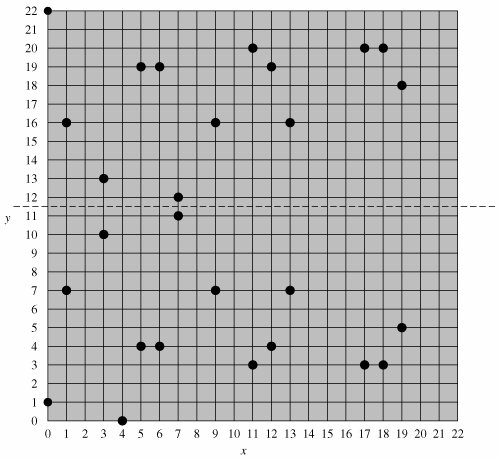
\includegraphics[scale=0.7]{images/ecczpexample.jpg}
\caption{Prime Elliptic Curve example}
\label{fig:ecczpexample}
\end{figure}

A finite abelian group can now be defined based on the set $E_{p}(a,b)$ provided that $(x^3 + ax + b) \bmod p)$ has no repeated factors. This is equivalent to the condition:

\begin{equation}
 (4a^3 + 27b^2) \bmod p \neq 0 \bmod p
 \label{eq:ecczpcon}
\end{equation}

which is of the same form as Equation \ref{eq:abrelecc}.

The rules for addition over $E_{p}(a,b)$ correspond to the algebraic technique described for elliptic curves defined over real numbers. For all points $P, Q \in E_{p}(a,b)$:

\begin{enumerate}
 \item $P + O + P$
 \item If $P = (x_{P},y_{P})$ then $P + (x_{P},-y_{P}) = O$ where $(x_{P},-y_{P}) = -P$
 \item If $P = (x_{P},y_{P})$ and $Q = (x_{Q},y_{Q})$ with $P \neq Q$, then $R = P + Q = (x_{R},y_{R}$ is calculated using:
	\[x_{R} = (\lambda^2 - x_{P} - x_{Q}) \bmod p \]
        \[ y_{R} = (\lambda(x_{P} - x_{R}) - y_{P}) \bmod p\]
 where
 \[ \lambda = \left\{
  \begin{array}{l l}
    \left( \frac{y_{Q} - y_{P}}{x_{Q} - x_{P}} \right) \bmod p & \quad \mathrm{if} P \neq Q \\
    \left(\frac{3x^{2}_{P} + a}{2y_{P}}\right) \bmod p & \quad \mathrm{if} P = Q
  \end{array} \right.
\]

 \item Multiplication is defined as repeat addition; for example $5P = P + P + P + P + P$
\end{enumerate}

\subsubsection{Description}

The following comparisons can be made between RSA and ECC, shown in Table \ref{tab:eccrsa}.

\begin{table}[htb]
\begin{center}
    \begin{tabular}{| l | l | }
    \hline
    RSA & ECC\\ \hline
    Modular multiplication & Addition operation \\ \hline
    Modular exponentiation & Multiple addition \\
    \hline
    \end{tabular}
   \caption{Comparison between RSA and ECC}
    \label{tab:eccrsa}
\end{center}
\end{table} 

Therefore, to create a cryptographic system using elliptic curves, a problem corresponding to the factoring of two large primes needs to be found. Considering the equation $Q = kP$ where $Q, P \in E_{P}(a,b)$ and $k < p$, it can be seen that it is relatively easy to calculate $Q$ given $k$ and $P$, but it is relatively hard to determine $k$ given $Q$ and $P$. This problem is called the discrete logarithm problem for elliptic curves. 

To illustrate this, take the group $E_{23}(9,17)$ which is defined by the equation

\[ y^2 \bmod 23 = (x^3 + 9x + 17) \bmod 23 \]

Taking the following values of $P$ and $Q$, the basis of the cipher with these parameters is; what is the discrete logarithm $k$ of $Q = (4,5)$ to the base $P = (16,5)$? A brute-force method to calculating $k$ would be to compute multiples of P until Q is found;

\[ P = (16,5), 2P = (20,20), 3P = (14,14), \]
\[ 4P = (19,20) ... 8P = (12,17), 9P = (4,5) \]

which shows $k = 9$. 

In practice, $k$ would be so large, a brute-force approach would be computationally infeasible. 

\paragraph{Key Generation}

Firstly, a prime integer $q$ and elliptic curve parameters $a$ and $b$ for Equation \ref{eq:mainecczpeq} are selected. This defines the elliptic group of points $E_{q}(a,b)$. A base point $G = (x_{1},y_{1}) \in E_{q}(a,b)$ whose order is a very large value $n$, where order $n$ of $G$ is the smallest positive integer $n$ such that $nG = 0$. $G$ and $n$ are global public elements, known to all participants. 

User A creates their private key by selecting an integer $n_{A}$, less than $n$. They can then generate their public key $P_{A} = n_{A} \times G$. This public key is a point in $E_{q}(a,b)$. User B creates their private ($n_{B}$) and public ($P_{B} = n_{B} \times G$) keys in the same way.

\paragraph{Encryption}

Encryption begins by encoding the plaintext message $m$ as an $x-y$ point $P_{m}$. As not all coordinates are in $E_{q}(a,b)$, the message cannot just be simply encoded into an $x-y$ point. The point $P_{m}$ will be encrypted as ciphertext and sent to the recipient to be decrypted. 

For user A to encrypt and send the message $P_{m}$ to user B, A chooses a random positive integer $k$ and uses B's public key $P_{B}$ to produce the ciphertext $C_{m}$ as a pair of points:

\[ C_{m} = \{kG , P_{m} + kP_{B}\} \]

\paragraph{Decryption}

To decrypt the ciphertext $C_{m}$ above, B multiplies the first point in the pair by their private key and subtracts the result from the second point:

\[ [P_{m} + kP_{B}] - [n_{B}(kG)] = P_{m} + k(n_{B}G) - n_{B}(kG) = P_{m} \]

The message $P_{m}$ has been obscured by A through the addition of $kP_{B}$. Only A knows the value of K, so even though $P_{B}$ is public, no-one can remove the $kP_{B}$. If someone knows the private key $n_{B}$, however, the 'clue' $kG$ (included by A) can be utilised. For an attacker to recover the message, they would have to compute $k$ given $G$ and $kG$, which is assumed to be (very) hard. 

Now that B knows the point $P_{m}$, they can decode the message using the already agreed upon coding method to retrieve the plaintext message $m$.

\subsubsection{Example}

A basic example will now be completed to demonstrate the encryption process. 

Firstly, take 

\[p = 751 \: \: \mathrm{and} \: \: E_{P}(-1,188)\]

which is equivalent to the curve 

\[y^2 = x^3 - x + 188\]

 Also take $G = (0,37)$.

For A to send a message to B, A first encodes the message into the elliptic point $P_{m} = (562,201)$ and selects the random number $k = 386$. As B's public key is $P_{B} = (201,5)$, the process continues as follows:

\[ kG = 386(0,376) = (676,558) \]
\[ P_{m} + kP_{B} = (562,201) + 386(201,5) = (385,328) \]

Thus, A sends the ciphertext

\[ C_{m} = \{(676,558),(385,328)\} \]

\subsubsection{Summary}

Elliptic Curve Cryptography is an asymmetric encryption scheme which operates with a global public elements $E_{q}(a,b)$ (elliptic curve group) and $G$ (point on elliptic curve with large order $n$

The keys used for this scheme are

\[PR = \{n_{B}\} \]\[PU = \{P_{B} = n_{B} \times G\} \]

and similarly for user B.

Encryption is completed to generate the cipher text $C_{m}$ by:

\[ C_{m} = \{kG , P_{m} + kP_{B}\} \]

with decryption taking place as follows

\[ [P_{m} + kP_{B}] - [n_{B}(kG)] = P_{m} + k(n_{B}G) - n_{B}(kG) = P_{m} \]

An encoding is required to transform the input plaintext message $m$ into a point $P_{m}$ in the established elliptic group.


\section{Comparison Factors}

As the third section of this project is centred around the analysis and comparison of the various cryptographic schemes implemented through the software development, research was performed in order to discover which factors contribute to how successful or useful the implemented schemes are. Most of the discovered factors were found in the article by Nirav Jobanputra, \textit{et al} \cite{ejeta}. This article studies not only the comparisons of various cryptographic techniques when implemented on a smartphone, but also Bio-information based security solutions such as finger-printing or voice recognition. However, the article was published in 2009 and has therefore the conclusions have lost some relevance due to the multitude of advancements that have been made regarding smartphones. 

That comparison factors that were found that could be used when analysis and concluding the results of this project were:

\begin{itemize}
 \item \textbf{Difficulty of techniques required to break encryption} - Level of various cryptanalytic techniques required to break the encryption. 
 \item \textbf{Battery usage} - Percent of battery usage for the duration of the application completing its required tasks. 
 \item \textbf{Key generation time} - The time it takes to generate the particular key.
 \item \textbf{Encryption and Decryption time} - The time it takes from start to finish to encrypt and decrypt a particular controlled file. 
 \item \textbf{Cryptographic key size} - Size of the key required for the particular cryptographic technique. 
 \item \textbf{Data usage} - Amount of data that is stored by the application and the amount of data that is sent or received. 
 \item \textbf{Application size} - Size of the application once it has been installed on the smartphone. 
 \item \textbf{Number of server connections} - The number of times any sort of data needs to be sent from the server to the phone or the converse.   
\end{itemize}

A combination of these comparison factors will be used to fully compare and contrast all aspects of the cryptographic schemes that will be implemented in this project. 

\section{Conclusion}

The results of the research completed for this project has now been presented in full. Research material was mostly found through the Warwick University library and online database, in the form of textbooks, e-books and online papers or articles. As mentioned, the Google play marketplace was used to research the various Android applications. Keywords such as 'Cryptography' and 'Encryption' where used to search the databases, as well as many others relating to the field off study in which research was being completed. The outcome of the research forms the backbone of the project and is of such a quality that the project can continue from this point very successfully. This is through the depth and breadth of information and knowledge gained from the research as a result of large and thorough research material databases and stores. The materials used are from reliable and prominent authors and the information was consistently found in other texts or forms when cross-checking and verifying the material. Chapters or sections of use were found directly, as opposed to reading the whole material from start to finish being required. This is due to the fact that the topic and required outcomes of each section of research was known before hand and allowed the next section of research to be more focused.

As a result of this research, a full system can be designed and implemented to allow for the generation of the results required to answer the main questions and problems specified in this project and to reach specific conclusions and outcomes.  

\chapter{Design}

\section{Introduction}

Within this section a full system overview will be given, accompanied by a more in-depth description of each of the main parts of the system. This will include the; Server, Database, Clients (P.C and Android) and the key sharing protocol. Diagrams will add in the description of the designed system and will be of the form of Unified Modeling Language (UML) diagrans. UML diagrams are based upon a set of graphic notation techniques used to deponstrate visually object-orientated software systems, found particularly described in the book by Minh Duc Bui \cite{umlbook}.

\section{Objectives}

The objectives of the design phase of this project can be found in the main 'Objectives' section of this report. However, to reiterate the development specific objectives in an alternate form and in light of the research completed;

\begin{enumerate}
 \item Develop a data communication framework, which includes;

    \begin{enumerate}
      \item Server
      \item Database
      \item Mobile Application
      \item P.C Client
    \end{enumerate}

  \item Design and implement cryptographic techniques to allow for testing;

    \begin{enumerate}
      \item Key exchange protocol
      \item RSA
      \item AES
    \end{enumerate}

\end{enumerate}

How these goals will be achieved will be covered throughout this section.

\section{Main System}

\subsection{Overview}

Put simply, the system to be created is a multi-client server facilitating the communication of data between two clients. The data is encrypted (and decrypted) using different cryptographic schemes. Figure \ref{fig:mainsystem1} shows a basic design of the system and how the main sections will interact. The server is the central controlling program (as opposed to a hardware system) communicating with each other piece of the overall system; the database to save, edit or retrieve user data and the clients to send and transfer data messages to other clients of the system.

\begin{figure}[htb]
\centering
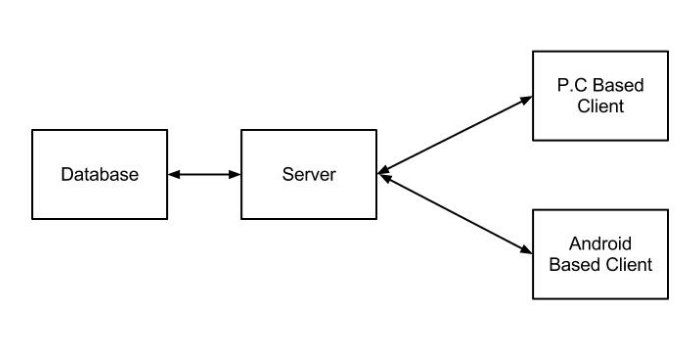
\includegraphics[scale=0.4]{images/mainsystem1.jpg}
\caption{Basic System Design}
\label{fig:mainsystem1}
\end{figure}

In order to fully explain the system, each system module will now be taken and explained in detail individually. 

\subsection{Server}

The primary purpose of the server is to facilitate the sending of messages between any two users of the system. A connection is formed between a client and the server via sockets, with an independent socket connection for each client that is currently communicating with the server. The server has full access to the accompanying database, with permission to query or edit database entries. Connection by the server to the database is managed through a database management class. 

The server has the ability to save required files in it's own associated disk space. The files saved by the server will be:

\begin{itemize}
 \item Message response files e.g. 'no new message' files.
 \item Transmission acknowledgement files.
 \item Encrypted messages to be sent to clients.
 \item Cryptographic keys belonging to the server and the clients that have completed the exchange protocol. 
\end{itemize}

Files received from the users of the system will be named using the following template, before being saved, to create a structure file system which will allow for the quick and simple finding of any required files. 

\begin{center}
 \textit{to/from ID Day Month Time(hh mm ss GMT) year.xml} \\
 e.g. from user8 Mon Mar 04 10 48 GMT 2013.xml
\end{center}

Once a socket connection between the server and client, the client user is required to 'sign in' to verify that they have a user account set up with the system already. Once the user has signed in, any messages that the server has waiting to be sent to current user, can then be sent. The 'signing in' protocol, from the point of view of the server, is as follows:

\begin{algorithm}
\caption{Client log in protocol}
\label{alg:loginprot}
\begin{algorithmic}
\State Is the client a user?
\If {client is a system user}
    \State What is the users ID?
    \If {ID exists in database}
      \State User logged into system
    \Else 
      \State ID doesn't exist - restart protocol
    \EndIf
\Else
   \If {User IP address matches a user database entry}
      \State Client is a system user
      \State Log in that user ID
    \Else
      \State Create a new user entry in the database
      \State Log in the new user
    \EndIf
\EndIf

\State Send to the user any waiting messages found in the database
\State Receive recipient user ID and message from logged in user and save to database

\end{algorithmic}
\end{algorithm}

This protocol fully satisfies the needs of this project. A few alterations would need to be made if the system were to be released to the public. To ensure user account security, a log in password should be required and requested of user when their account is set up and each time they wish to log in. A more unique form of separate identification should be used to reinforce the individual identification number, for example their verified email address, as opposed to the I.P address used above. However, these points do not pose an issue for this project, as the system is created in order to answer specific questions, not as a product to release to the public. 

Another important feature of the server is that it acts as a trusted third party within the cryptographic process. It has its own associated public and private keys so that encrypted messages between the server and the client can be sent. If only the clients key was used, encrypted messages could only be sent from the server to the client and not from the client to the server. The importance of this feature will become more apparent in the key exchange protocol description. 

\subsection{Database}

The database for this project is built using the MySQL database management system, as described previously, hosted on the 'local host'. This enables the database to be used with the local server, without having to host both the database and server on an external host, which incurs sizeable costs as no completely free hosting exists. 

The design of the database is to store, for each user entry, the following information:

\begin{itemize}
 \item\begin{description}
   \item[Unique ID] An ID assigned to each user which is individual and different to all other users 
 \end{description} 
 \item\begin{description}
   \item[I.P Address] The I.P address of the user 
 \end{description}
 \item\begin{description}
   \item[Pubic Key location] The disk location of the users public key, stored and used by the server 
 \end{description}
 \item\begin{description}
   \item[Message Location] The storage location of the next message waiting to be sent to the user
 \end{description}
 \item\begin{description}
   \item[Key Exchange file locations] Locations of the files used for the key exchange protocol 
 \end{description}
\end{itemize}


The Unique ID acts as the primary key, which is used to uniquely identify each record in the database table. The ID is automatically generated by the database management system when a new user is added to the database, escaping the possibility of human error, and consists of a positive integer. The assignment of the primary key is based on an incremented counter, so if an entry is deleted from the table, that user ID will not be used again.

To expand this database to allow for an increased user base than the one in which this project is operating with, another relational database table would be created to store all of the messages in the system, accompanied with the User ID of the recipient of that message. When a user logs into the system, the server would query the database and return all of the messages from the appropriate database intended for that user. However, this is a featured not required in this project, but is worth mentioning in preparation for the 'Further Work' section. 

As mentioned previously, the database is managed by the server through the use of a database management class. This class is responsible for connecting to the hosted database and querying data entries, among other tasks. The class diagram for this module can be seen in Figure \ref{fig:dbmanclass}

\begin{figure}[htb]
\centering
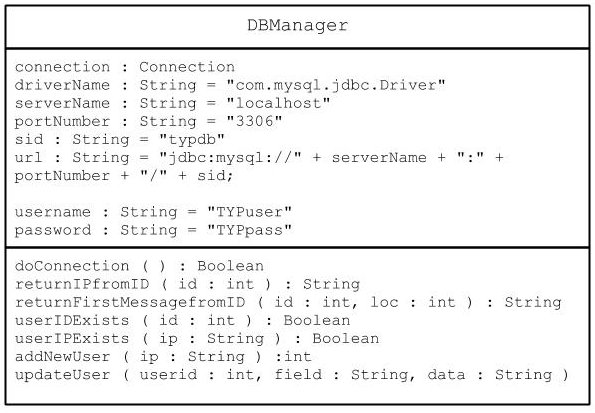
\includegraphics[scale=0.4]{images/dbmanagerclass.jpg}
\caption{UML Class diagram for the DBManager class}
\label{fig:dbmanclass}
\end{figure}

\subsection{Clients}

The clients are how the users of the system interact and operate the system and act as a mirror image of the server. During the log in protocol, the server requires the users log in ID. This is mirrored for the client in the request for the user to input their user ID. The user wishes to send a message to another user, so enters the recipient ID and message. This is mirror for the server by the receiving of the recipient ID and message, which the server saves at a specified location on disk and in the corresponding database entry. The client also allows the data sent to the server to be encrypted and can decrypt data sent to the client. These requirements of the client are better represented in the following list which outlines the capabilities of the designed client:

\begin{itemize}
 \item Connects to the server via sockets
 \item Generates and stores its own keys
 \item Specify which other client the user wishes to send a data message to
 \item Retrieve the data message input from the user
 \item Complete the key exchange protocol required
 \item Encrypt the message to be sent
 \item Send the encrypted, user input, data messages to the server
 \item Receive encrypted messages from the server
 \item Decrypt and present to the user the received message
\end{itemize}

The client class contains the methods and protocols allowing it to complete the above tasks. The P.C client and Android application inherit these abilities from the client but are more specific, so are implemented according to their own rules and requirements. For example, to ensure the operation of the application does not noticeably impact the functionality of visual performance of the smartphone, socket connections and data transfer will be performed as an asynchronous, background, task. This allows a P.C client to send a message, via the server, to another P.C client or an android application client. Different encryption (and decryption) methods can be implemented through a different instance of the P.C or android clients. For example, in Figure \ref{fig:clienthier}, Application 1 and P.C Client 1 implement a particular scheme and Application 2 and P.C Client 2 implement a different encryption scheme. So, P.C Client 1 has all the capabilities of P.C Client, with an added encryption method and so on for the other instances of P.C and Android Clients shown in the diagram. 

\begin{figure}[htb]
\centering
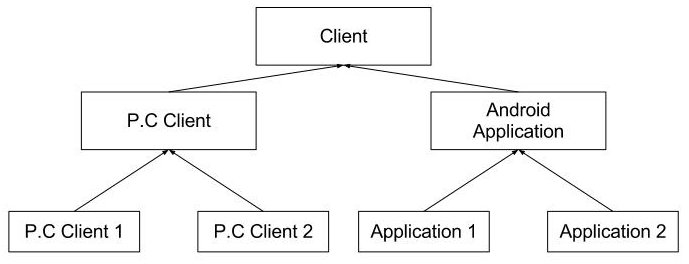
\includegraphics[scale=0.4]{images/designs2.jpg}
\caption{Basic inheritance hierarchy of the clients}
\label{fig:clienthier}
\end{figure}

Compatibility between the P.C and Android based clients will be ensured through the use of the XML file structure. Figure \ref{fig:xmldesign} shows the design of the XML file that will contain all the data required for the message to be sent and received.  

\begin{figure}[htb]
\centering
\lstinputlisting[basicstyle=\ttfamily\scriptsize]{documents/xmldesign.xml}
\caption{XML file layout.}
\label{fig:xmldesign}
\end{figure}

The XML file creation and parsing (data retrieval) will be managed by separate management classes, instances of which will be used by each client. Figure \ref{fig:xmlclass} displays the UML class diagrams for these designed classes.

\begin{figure}[htb]
\centering
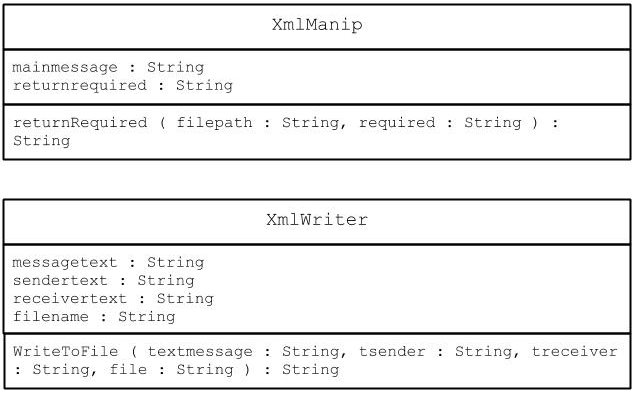
\includegraphics[scale=0.4]{images/xmlclass.jpg}
\caption{UML Class diagrams for the XML management classes}
\label{fig:xmlclass}
\end{figure}

\appendix
\chapter{Gantt Chart}\label{A}
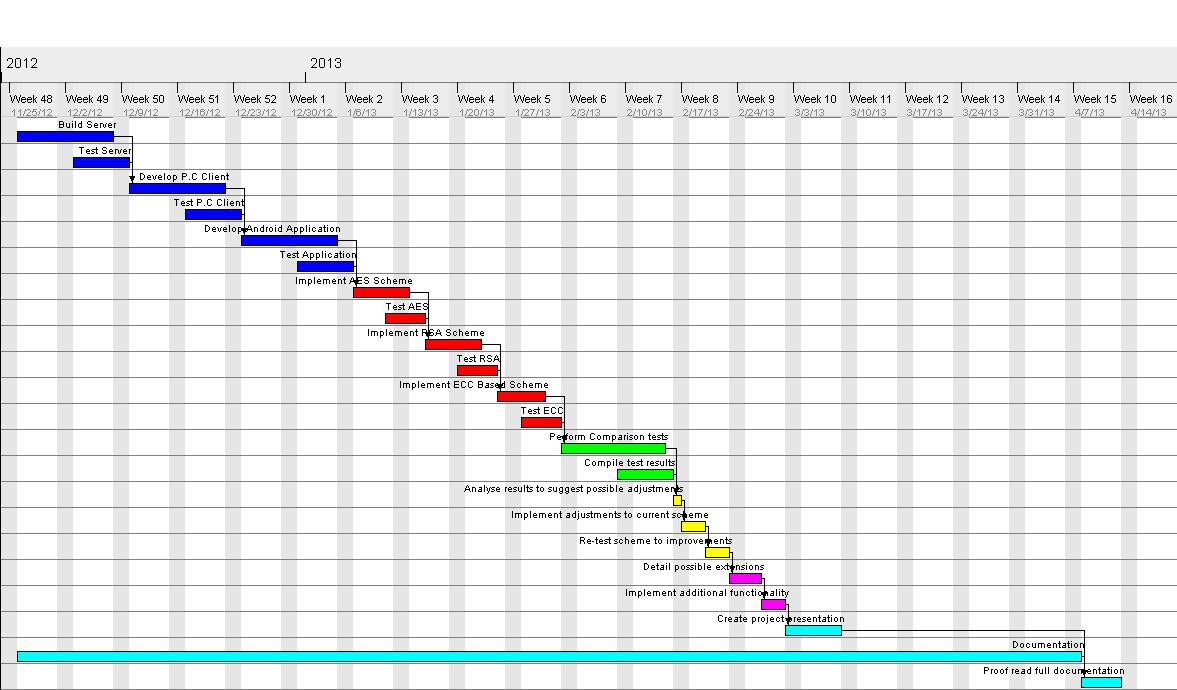
\includegraphics[scale=0.35, angle=270]{images/ProgReportChart.jpg}

\bibliography{projectbib}

\end{document}          